\documentclass{article}
\usepackage[utf8]{inputenc}
\usepackage{amsmath}
\usepackage{amssymb}
\usepackage{amsthm}
\usepackage{graphicx}
% \usepackage[ngerman]{babel}

\begin{document}

% Aufgabe
\subsection*{Aufgabe}
Für $c>0$ betrachte die \emph{logarithmische Spirale}
$f:(-\infty,0]\to\mathbb{R}^2$,  
$$
   f(t) := (e^{ct}\cos t,e^{ct}\sin t).
$$
(a) Zeichne die Kurve $f$.

(b) Berechne die Länge von $f$.

\subsection*{Lösung}

\textbf{(a) Zeichnung der Kurve}

Die logarithmische Spirale $f(t) = (e^{ct}\cos t, e^{ct}\sin t)$ für $t \in (-\infty, 0]$ hat folgende Eigenschaften:

\begin{itemize}
\item Für $t \to -\infty$ gilt $e^{ct} \to 0$ (da $c > 0$), also nähert sich die Kurve spiralförmig dem Ursprung $(0,0)$.
\item Für $t = 0$ erhalten wir $f(0) = (e^0\cos 0, e^0\sin 0) = (1, 0)$.
\item Die Kurve windet sich gegen den Uhrzeigersinn um den Ursprung, da $t$ von $-\infty$ nach $0$ wächst.
\item Der Faktor $e^{ct}$ sorgt für das exponentielle Wachstum des Abstands zum Ursprung.
\end{itemize}

\begin{figure}[h]
\centering
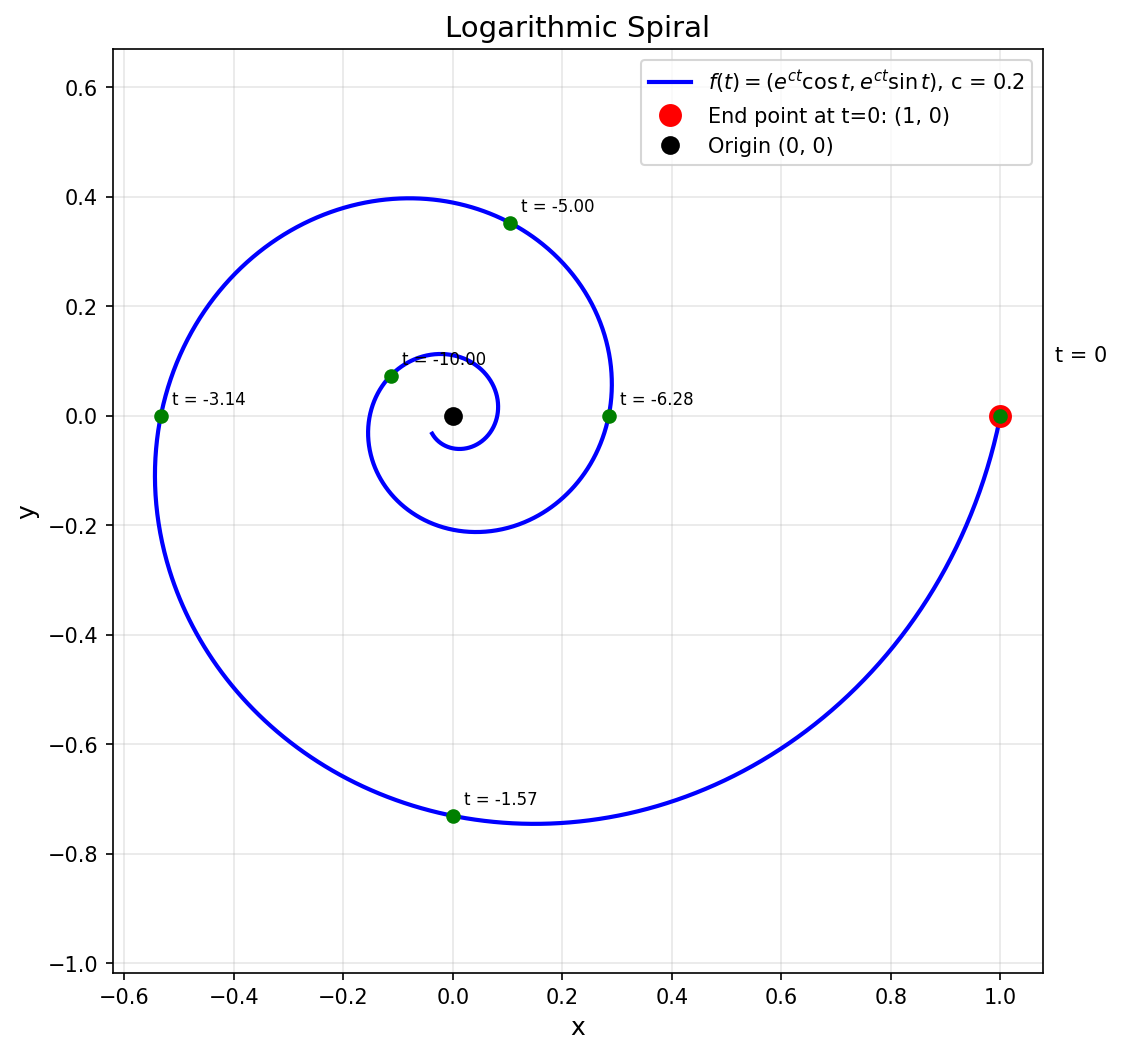
\includegraphics[width=0.8\textwidth]{logarithmic_spiral_detailed.png}
\caption{Logarithmische Spirale für $c = 0.2$. Die Kurve beginnt bei $t \to -\infty$ im Ursprung und endet bei $t = 0$ im Punkt $(1, 0)$.}
\end{figure}

\textbf{(b) Berechnung der Länge}

Die Länge einer parametrisierten Kurve $f: [a,b] \to \mathbb{R}^2$ ist gegeben durch:
$$L = \int_a^b |f'(t)| \, dt$$

Zunächst berechnen wir die Ableitung $f'(t)$:
\begin{align}
f(t) &= (e^{ct}\cos t, e^{ct}\sin t)\\
f'(t) &= \left(\frac{d}{dt}(e^{ct}\cos t), \frac{d}{dt}(e^{ct}\sin t)\right)
\end{align}

Für die einzelnen Komponenten erhalten wir mit der Produktregel:
\begin{align}
\frac{d}{dt}(e^{ct}\cos t) &= ce^{ct}\cos t - e^{ct}\sin t = e^{ct}(c\cos t - \sin t)\\
\frac{d}{dt}(e^{ct}\sin t) &= ce^{ct}\sin t + e^{ct}\cos t = e^{ct}(c\sin t + \cos t)
\end{align}

Nun berechnen wir $|f'(t)|^2$:
\begin{align}
|f'(t)|^2 &= \left(\frac{dx}{dt}\right)^2 + \left(\frac{dy}{dt}\right)^2\\
&= e^{2ct}(c\cos t - \sin t)^2 + e^{2ct}(c\sin t + \cos t)^2\\
&= e^{2ct}\left[(c\cos t - \sin t)^2 + (c\sin t + \cos t)^2\right]
\end{align}

Wir expandieren die Klammern:
\begin{align}
(c\cos t - \sin t)^2 &= c^2\cos^2 t - 2c\cos t \sin t + \sin^2 t\\
(c\sin t + \cos t)^2 &= c^2\sin^2 t + 2c\sin t \cos t + \cos^2 t
\end{align}

Die Summe ergibt:
\begin{align}
&(c\cos t - \sin t)^2 + (c\sin t + \cos t)^2\\
&= c^2\cos^2 t - 2c\cos t \sin t + \sin^2 t + c^2\sin^2 t + 2c\sin t \cos t + \cos^2 t\\
&= c^2(\cos^2 t + \sin^2 t) + (\sin^2 t + \cos^2 t)\\
&= c^2 \cdot 1 + 1\\
&= c^2 + 1
\end{align}

Somit ist:
$$|f'(t)|^2 = e^{2ct}(c^2 + 1)$$

und daher:
$$|f'(t)| = e^{ct}\sqrt{c^2 + 1}$$

Die Länge der Kurve ist nun:
\begin{align}
L &= \int_{-\infty}^0 |f'(t)| \, dt\\
&= \int_{-\infty}^0 e^{ct}\sqrt{c^2 + 1} \, dt\\
&= \sqrt{c^2 + 1} \int_{-\infty}^0 e^{ct} \, dt
\end{align}

Wir berechnen das Integral:
\begin{align}
\int_{-\infty}^0 e^{ct} \, dt &= \left[\frac{e^{ct}}{c}\right]_{-\infty}^0\\
&= \frac{e^{c \cdot 0}}{c} - \lim_{t \to -\infty} \frac{e^{ct}}{c}\\
&= \frac{1}{c} - 0\\
&= \frac{1}{c}
\end{align}

Dabei haben wir benutzt, dass $\lim_{t \to -\infty} e^{ct} = 0$ für $c > 0$.

Die Gesamtlänge der logarithmischen Spirale ist somit:
$$\boxed{L = \frac{\sqrt{c^2 + 1}}{c}}$$

\end{document}